\newcommand{\imageScale}{0.2}

\tikzset{%
  >={Latex[width=2mm,length=2mm]},
  % Specifications for style of nodes:
            base/.style = {rectangle, rounded corners, draw=black,
                           minimum width=\width, minimum height=1cm,
                           text centered},
            red/.style = {base, fill=red!15},
            blue/.style = {base, fill=blue!15}}
          

\begin{center}
\begin{tikzpicture}[node distance=1.5cm, every node/.style={fill=white}, align=center]

	\node(User)[xshift=-10cm]{\includegraphics[scale=\imageScale]{User}};		
	\node(UserText)[below of=User]{User};		
	
	\node(GUI)[base, right of=User, xshift=(\width), yshift=2cm]{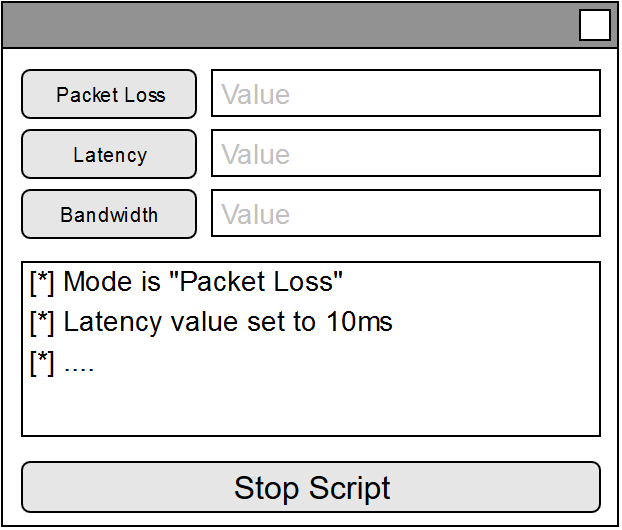
\includegraphics[scale=\imageScale]{Packet_UI_Design}};
	\node(GUIText)[below of=GUI, yshift=-0.5cm]{GUI};	
	
	\node(CLI)[base, below of=GUI, yshift=-2.25cm]{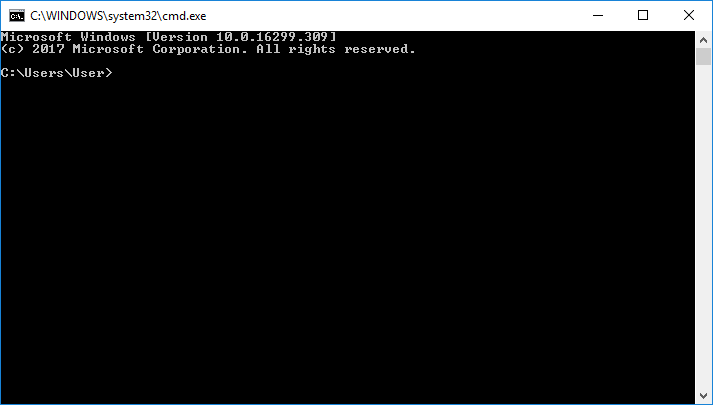
\includegraphics[scale=\imageScale]{CLI}};
	\node(CLIText)[below of=CLI]{CLI};
	
	\node(Effect)[blue, right of=User, xshift=(\width * 2) + 2cm]{Effect Choice};	
	\node(Nfqueue)[base, right of=Effect, xshift=(\width)]{NFQUEUE Creation};	
	
	\node(Parameters)[base, below of=Effect]{Parameter Handling};	
		
	
	\node(Packet)[red, below of=User, xshift=2cm, yshift=-4cm, text width=6cm]{Incomming Packets pushed into the NFQUEUE};
	\node(ChosenEffect)[blue, right of=Packet, xshift=\width + 2cm]{Chosen Effect};
	\node(PacketDescription)[above of=Packet, yshift=-0.5cm]{{\bf While NFQUEUE is running}};
	
	\draw[->] (User)--(GUI);
	\draw[->] (User)--(CLI);
	
	\draw[->] (GUI)--(Effect);
	\draw[->] (CLI)--(Parameters);
	\draw[->] (Parameters)--(Effect);	
	
	\draw[->] (Effect)--(Nfqueue);
	\draw[->] (Packet)--(ChosenEffect);
		
\end{tikzpicture}
\end{center}